\documentclass{article}
\usepackage{ctex}
\usepackage{tikz}
\usetikzlibrary{arrows.meta} % 引入一些箭头
\usepackage{pgfplots} % 引入绘图宏包
\usepackage{tcolorbox}
\begin{document}
% \section{三角函数}
% 

这是默认的配置\\
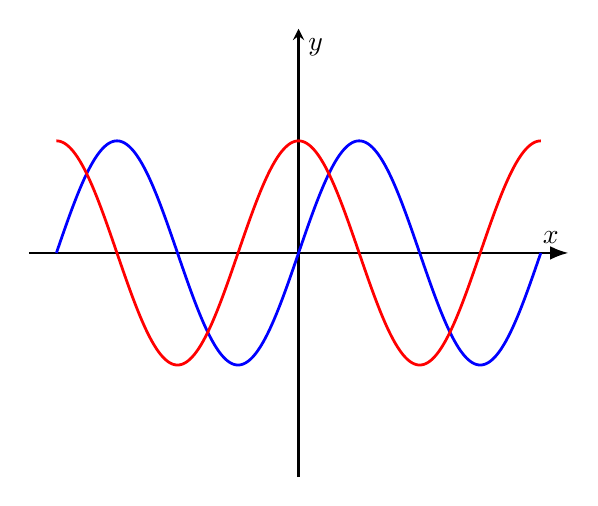
\begin{tikzpicture}
    \begin{axis}[
        axis lines = middle,%将坐标系的 x 轴和 y 轴放置在图形区域的中央(原点位置),而不是默认的底部和左侧。
        xlabel = $x$,
        ylabel = $y$,
        xmin = -7,
        xmax = 7,
        ymin = -2,
        ymax = 2,
        clip = false, % 设置不裁剪图形,也就是函数图像会超过坐标轴的范围
        axis line style={thick}, %使坐标轴变粗
        x axis line style={-Latex},
        y axis line style={-stealth},
        % title = {设置$x$、$y$轴长度不同,但是图像上长度相同},   
        xtick=\empty,
        ytick=\empty %取消刻度
    ]
    \addplot [
        domain=-2*pi:2*pi ,
        samples=500,
        line width = 1pt,
        color=blue
    ]{(sin(deg(x)))};

    \addplot [
        domain=-2*pi:2*pi ,
        samples=500,
        line width = 1pt,
        color=red
    ]{(cos(deg(x)))};
    \end{axis}
\end{tikzpicture}

使用了 \verb|axis equal|让函数图像变成了原有的长度

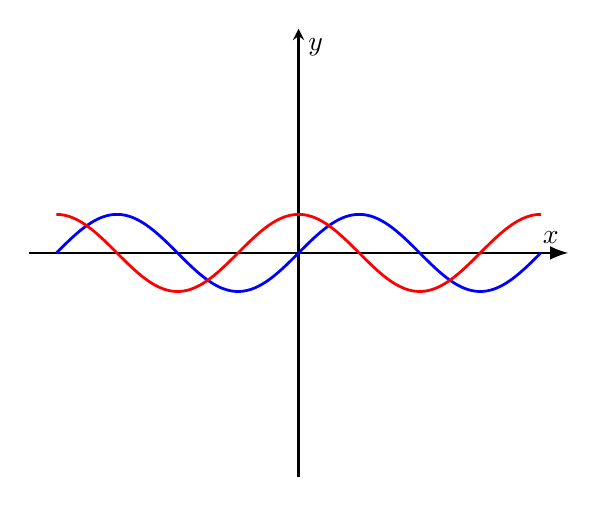
\begin{tikzpicture}
    \begin{axis}[
        axis lines = middle,%将坐标系的 x 轴和 y 轴放置在图形区域的中央(原点位置),而不是默认的底部和左侧。
        xlabel = $x$,
        ylabel = $y$,
        xmin = -7,
        xmax = 7,
        ymin = -2,
        ymax = 2,
        axis equal	,
        clip = false, % 设置不裁剪图形,也就是函数图像会超过坐标轴的范围
        axis line style={thick}, %使坐标轴变粗
        x axis line style={-Latex},
        y axis line style={-stealth},
        xtick=\empty,
        ytick=\empty %取消刻度
    ]
    \addplot [
        domain=-2*pi:2*pi ,
        samples=500,
        line width = 1pt,
        color=blue
    ]{(sin(deg(x)))};

    \addplot [
        domain=-2*pi:2*pi ,
        samples=500,
        line width = 1pt,
        color=red
    ]{(cos(deg(x)))};
    \end{axis}
\end{tikzpicture}






\begin{tikzpicture}
    \begin{axis}[
        axis lines = middle,%将坐标系的 x 轴和 y 轴放置在图形区域的中央(原点位置),而不是默认的底部和左侧。
        xlabel = $x$,
        ylabel = $y$,
        xmin = -7,
        xmax = 7,
        ymin = -2,
        ymax = 2,
        axis equal	,
        clip = false, % 设置不裁剪图形,也就是函数图像会超过坐标轴的范围
        axis line style={thick}, %使坐标轴变粗
        x axis line style={-Latex},
        y axis line style={-stealth},
        xtick=\empty,
        ytick=\empty %取消刻度
    ]
    \addplot [
        domain=-2*pi:2*pi ,
        samples=500,
        line width = 1pt,
        color=blue
    ]{(sin(deg(x)))};
    \end{axis}
\end{tikzpicture}



给 \verb|tikzpicture| 使用了标题
\begin{tcolorbox}
    \begin{tikzpicture}
        \begin{axis}[
            axis lines = middle,
            xlabel = $x$,
            ylabel = $y$,
            xmin = -7,
            xmax = 7,
            ymin = -2,
            ymax = 2,
            axis equal,
            clip = false,
            axis line style={thick},
            x axis line style={-Latex},
            y axis line style={-stealth},
            xtick=\empty,
            ytick=\empty,
            % 添加标题(全局标题,位于坐标轴上方)
            title = {$y = \sin(x)$ 函数图像}, % 用 $ 包裹可插入数学公式
            title style={font=\large, color=blue} % 可选:设置标题字体样式
        ]
        \addplot [
            domain=-2*pi:2*pi ,
            samples=500,
            line width = 1pt,
            color=blue
        ]{(sin(deg(x)))};
        \end{axis}
    \end{tikzpicture}
\end{tcolorbox}





使用 \verb|title| 来添加标题

\begin{tcolorbox}
    \begin{tikzpicture}
        \begin{axis}[
            axis lines = middle,
            xlabel = $x$,
            ylabel = $y$,
            xmin = -7, xmax = 7,
            ymin = -2, ymax = 2,
            axis equal,
            clip = false,
            axis line style={thick},
            x axis line style={-Latex},
            y axis line style={-stealth},
            xtick=\empty, ytick=\empty,
            legend pos=north east, % 图例位置
            title = {添加图例}, % 用 $ 包裹可插入数学公式
            title style={font=\large, color=blue} % 可选:设置标题字体样式
        ]
        \addplot [
            domain=-2*pi:2*pi,
            samples=500,
            line width = 1pt,
            color=blue
        ]{(sin(deg(x)))};
        \addlegendentry{$y = \sin(x)$} % 添加图例
        \end{axis}
    \end{tikzpicture}
\end{tcolorbox}


使用\verb|\node| 确定 $y = \sin(x)$ 的位置 
\begin{tcolorbox}
    \begin{tikzpicture}
        \begin{axis}[
            axis lines = middle,
            xlabel = $x$,
            ylabel = $y$,
            xmin = -7, xmax = 7,
            ymin = -2, ymax = 2,
            axis equal,
            clip = false,
            axis line style={thick},
            x axis line style={-Latex},
            y axis line style={-stealth},
            xtick=\empty, ytick=\empty,
        ]
        \addplot [
            domain=-2*pi:2*pi,
            samples=500,
            line width = 1pt,
            color=blue
        ]{(sin(deg(x)))};
        
        % 在x=π/2处添加标注(对齐函数最高点)
        \node[above right, font=\large, color=black] 
              at (axis cs:{pi/2}, {sin(deg(pi/2))}) {$y = \sin(x)$};
              % axis cs: 是 PGFPlots 定义的 坐标轴坐标系统
              %与之相对的是 绘图坐标系统(如 (current bounding box))或 绝对坐标系统(如 (0,0) 表示页面左下角)
    
        \end{axis}
        
    \end{tikzpicture}
\end{tcolorbox}




% \section{指数函数}
\begin{tikzpicture}
    \begin{axis}[
        axis lines = middle,%将坐标系的 x 轴和 y 轴放置在图形区域的中央(原点位置),而不是默认的底部和左侧。
        xlabel = $x$,
        ylabel = $y$,
        xmin = -7,
        xmax = 7,
        ymin = -2,
        ymax = 10,
        clip = false, % 设置false不裁剪图形,也就是函数图像会超过坐标轴的范围
        axis line style={thick}, %使坐标轴变粗
        x axis line style={-Latex},
        y axis line style={-stealth},
        % title = {设置$x$、$y$轴长度不同,但是图像上长度相同},   
        xtick=\empty,
        ytick=\empty %取消刻度
    ]
    \addplot [
        domain=-6:3 ,
        samples=500,
        line width = 1pt,
        color=blue
    ]{(2^x)};

    % \addplot [
    %     domain=-3:6 ,
    %     samples=500,
    %     line width = 1pt,
    %     color=red
    % ]{((1/2)^x)};
    \end{axis}
\end{tikzpicture}

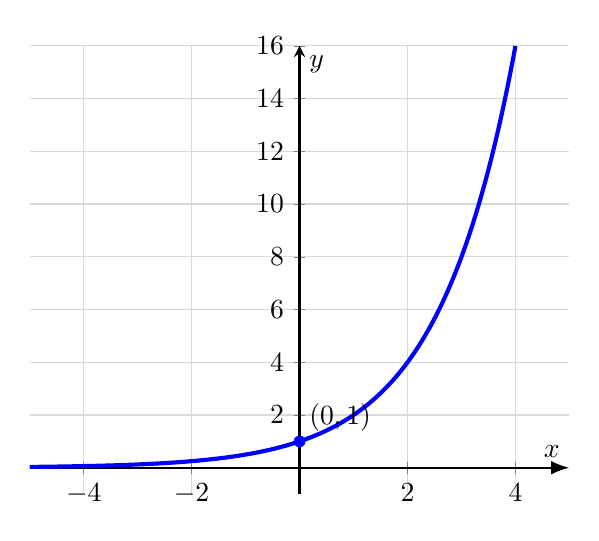
\begin{tikzpicture}
    \begin{axis}[
        axis lines = middle,
        xlabel = $x$,
        ylabel = $y$,
        xmin = -5,
        xmax = 5,
        ymin = -1,
        ymax = 16,
        clip = false,
        axis line style={thick},
        x axis line style={-Latex},
        y axis line style={-stealth},
        % title = {$y = 2^x$},
        xtick={-4,-2,0,2,4},
        ytick={2,4,6,8,10,12,14,16},
        grid=both,
        grid style={gray!30}
    ]
    \addplot [
        domain=-5:4,
        samples=200,
        line width = 1.5pt,
        color=blue,
        smooth
    ]{(2^x)};
    
    % 标记y轴截距 (0,1)
    \node[circle, fill=blue, inner sep=1.5pt] at (axis cs:0,1) {};
    \node[anchor=south west] at (axis cs:0,1) {$(0,1)$};
    % anchor=south west 节点的左下角与定位点 ⋆ 对齐,即(axis cs:0,1)
    \end{axis}
\end{tikzpicture}









\begin{tcolorbox}
    用虚线来判断底数\\
    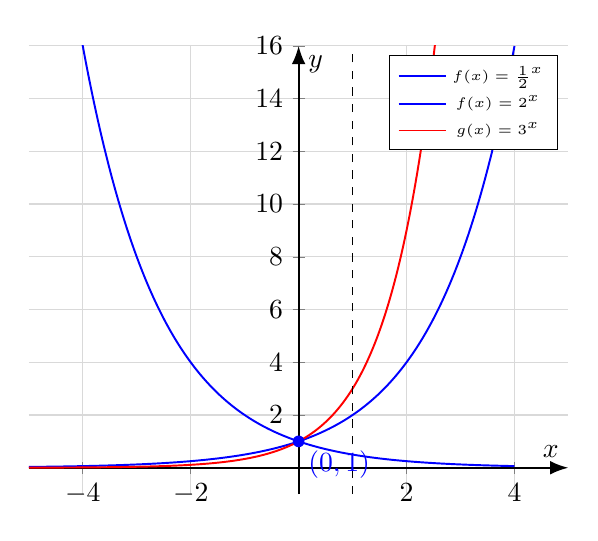
\begin{tikzpicture}[scale =1]
        \begin{axis}[ 
            axis lines = middle, %x 轴和 y 轴均穿过原点(0,0),将坐标系分为四个象限。
            xlabel = $x$,
            ylabel = $y$,
            xmin = -5,
            xmax = 5,
            ymin = -1,
            ymax = 16,
            clip = true,
            axis line style={thick},
            x axis line style={-Latex},
            y axis line style={-Latex},
            % title = {$y = 2^x$},
            xtick={-4,-2,0,2,4},
            ytick={2,4,6,8,10,12,14,16},
            grid=both,
            grid style={gray!30}
        ]
        \addplot [
            domain=-5:4,
            samples=200,
            line width = 0.7pt,
            color=blue,
            smooth
        ]{((1/2)^x)};
        \addlegendentry{\tiny $f(x)=\frac{1}{2}^x$}
    
    
        \addplot [
            domain=-5:4,
            samples=200,
            line width = 0.7pt,
            color=blue,
            smooth
        ]{(2^x)};
        \addlegendentry{\tiny $f(x)=2^x$}
    
        \addplot [
            domain=-5:4,
            samples=200,
            line width = 0.7pt,
            color=red,
            smooth
        ]{(3^x)};
    
        \addlegendentry{\tiny $g(x)=3^x$}
    
        % 绘制一条竖直的虚线,即 x = 1
        \draw [dashed, black] 
            (axis cs:1, \pgfkeysvalueof{/pgfplots/ymin})
            -- (axis cs:1, \pgfkeysvalueof{/pgfplots/ymax});
        
    
    
    
        % 标记y轴截距 (0,1)
        \node[circle, fill=blue, inner sep=1.5pt] at (axis cs:0,1) {};
        \node[blue,anchor=north west] at (axis cs:0,1) {$(0,1)$};
        % anchor=south west 节点的左下角与定位点 ⋆ 对齐,即(axis cs:0,1)
        \end{axis}
    \end{tikzpicture}
\end{tcolorbox}







\subsection{对数函数}



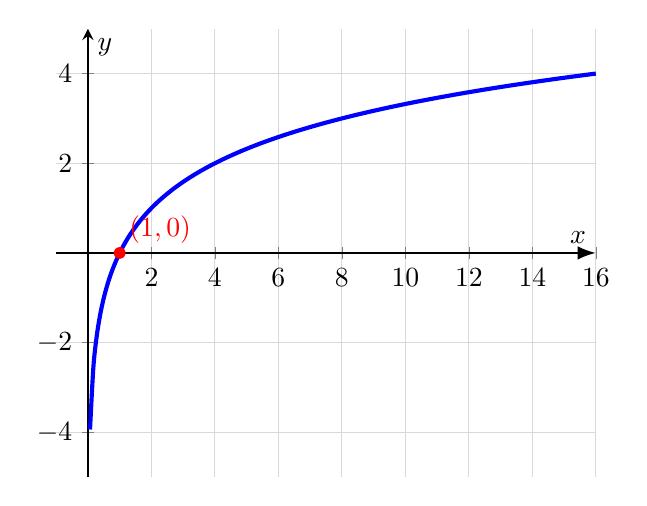
\begin{tikzpicture}
    \begin{axis}[
        axis lines = middle,
        xlabel = $x$,
        ylabel = $y$,
        ymin = -5,
        ymax = 5,
        xmin = -1,
        xmax = 16,
        clip = false,
        axis line style={thick},
        x axis line style={-Latex},
        y axis line style={-stealth},
        % title = {$y = 2^x$},
        ytick={-4,-2,0,2,4},
        xtick={2,4,6,8,10,12,14,16},
        grid=both,
        grid style={gray!30}
    ]
    \addplot [
        domain=-5:16,
        samples=200,
        line width = 1.5pt,
        color=blue,
        smooth
    ]{(ln(x)/ln(2))};
    
    % 标记y轴截距 (0,1)
    \node[circle, fill=red, inner sep=1.5pt] at (axis cs:1,0) {};
    \node[red,anchor=south west] at (axis cs:1,0) {$(1,0)$};
    % anchor=south west 节点的左下角与定位点 ⋆ 对齐,即(axis cs:0,1)
    \end{axis}
\end{tikzpicture}







\end{document}
